\documentclass[tikz,border=0pt]{standalone}
\usepackage{tikz}
\usepackage{booktabs}
\usepackage{pgfplots}
\usepackage{amsmath}
\pgfplotsset{compat=1.18}
\usepackage{subcaption}
\usepackage{caption}
\pagestyle{empty}
\begin{document}


% P-Sets per Layer — Poland_Warszawa_2018_Bialoleka_obszar_3.json
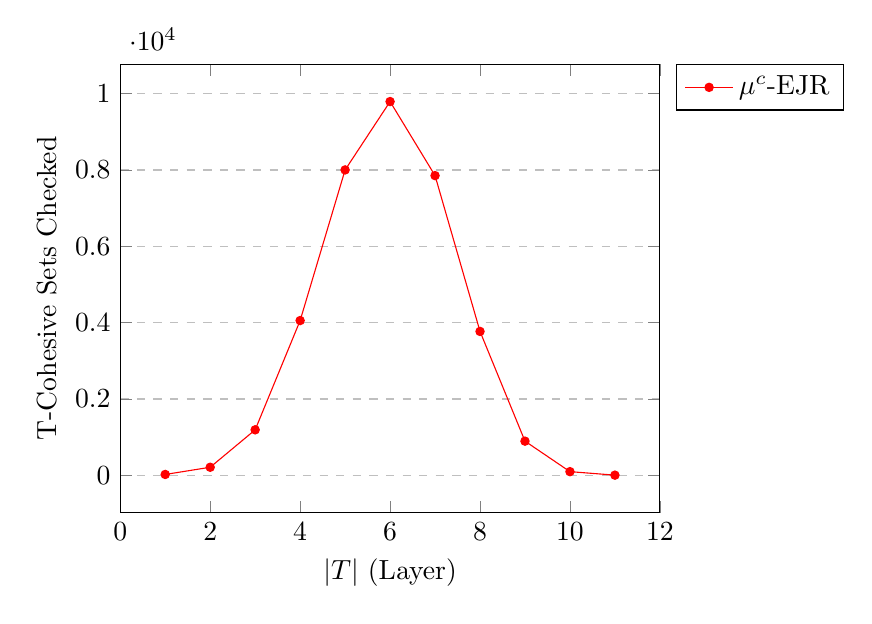
\begin{tikzpicture}
\begin{axis}[xlabel={$|T|$ (Layer)}, ylabel={T-Cohesive Sets Checked}, ymajorgrids=true, grid style=dashed, legend pos = outer north east]
\addplot[color=red, mark=*, mark size=1.5pt]coordinates { (1,21)(2,210)(3,1191)(4,4055)(5,8003)(6,9795)(7,7854)(8,3770)(9,894)(10,95)(11,3)};\addlegendentry{$\mu^c$-EJR}
\end{axis}
\end{tikzpicture}

\end{document}
